\title{Belegarbeit Computational Science and Engineering:\\
       Verteilte GPGPU-Berechnungen mit Spark }
\author {
	Maximilian Knespel
	\newline	\newline
	Betreuer: \and Dipl.-Inf. Nico Hoffmann
}
\date{}
%\date{7. Juli 2016}


\begin{document}

\begin{frame}
	\titlepage
\end{frame}

%\begin{frame}
%	\frametitle{Outline}
%	\setcounter{tocdepth}{1}
%	\tableofcontents
%\end{frame}


%%%%%%%%%%%%%%%%%%%%%%%%%%%%%%%%%%%%%%%%%%%%%%%%%%%%%%%%%%%%%%%%%%%%%%%%%%%%%%%%
\section{Einführung}
%%%%%%%%%%%%%%%%%%%%%%%%%%%%%%%%%%%%%%%%%%%%%%%%%%%%%%%%%%%%%%%%%%%%%%%%%%%%%%%%


\begin{frame}
    \frametitle{GPU-Beschleuniger zum Hochleistungsrechnen}
    % Bild K20x und AmdOpteron ? damit man sofort sieht, um was es auf der Folie geht?
    %  - https://commons.wikimedia.org/wiki/File:AMD_Opteron_2212_IMGP1795.jpg
    %  - http://images.nvidia.com/content/tesla/images/tesla-3-quater.png
    %
    % sagen:
    %   - Mittlerweile ist GPU an vielen Stellen schon Mainstream im Cluster-
    %     Computing geworden. Beispielhafter Beweis: die aktuelle Top 3 Titan XK7:
    %         18 688 AMD Opteron 6274 (16 Kerne)
    %         18 688 Nvidia Tesla K20X (90% der Rechenlast)
    %       https://www.olcf.ornl.gov/titan/
    %     und viele andere haben auch schon oder wollen aufrüsten
    %     Top 8 will dieses Jahr mit 4500 Pascal GPUs (16nm HBM2) aufrüsten
    %       http://nvidianews.nvidia.com/news/nvidia-pascal-gpus-to-double-speed-of-europe-s-fastest-supercomputer
    %     https://www.top500.org/lists/2016/06/
    %     http://on-demand.gputechconf.com/supercomputing/2012/presentation/SB005-Bland-Titan-Oak-Ridge-National-Labs.pdf
    %
    \begin{columns}
        \begin{column}
            \begin{center}
                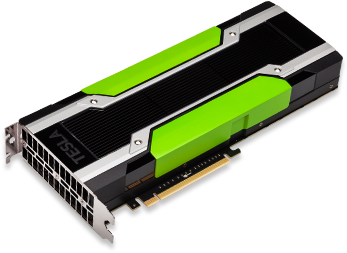
\includegraphics[height=0.1\textheight]{tesla-3-quater.png}
            \end{center}
            \textcolor{gray}{\scriptsize{NVIDIA}}
        \end{column}\begin{column}
            \begin{center}
                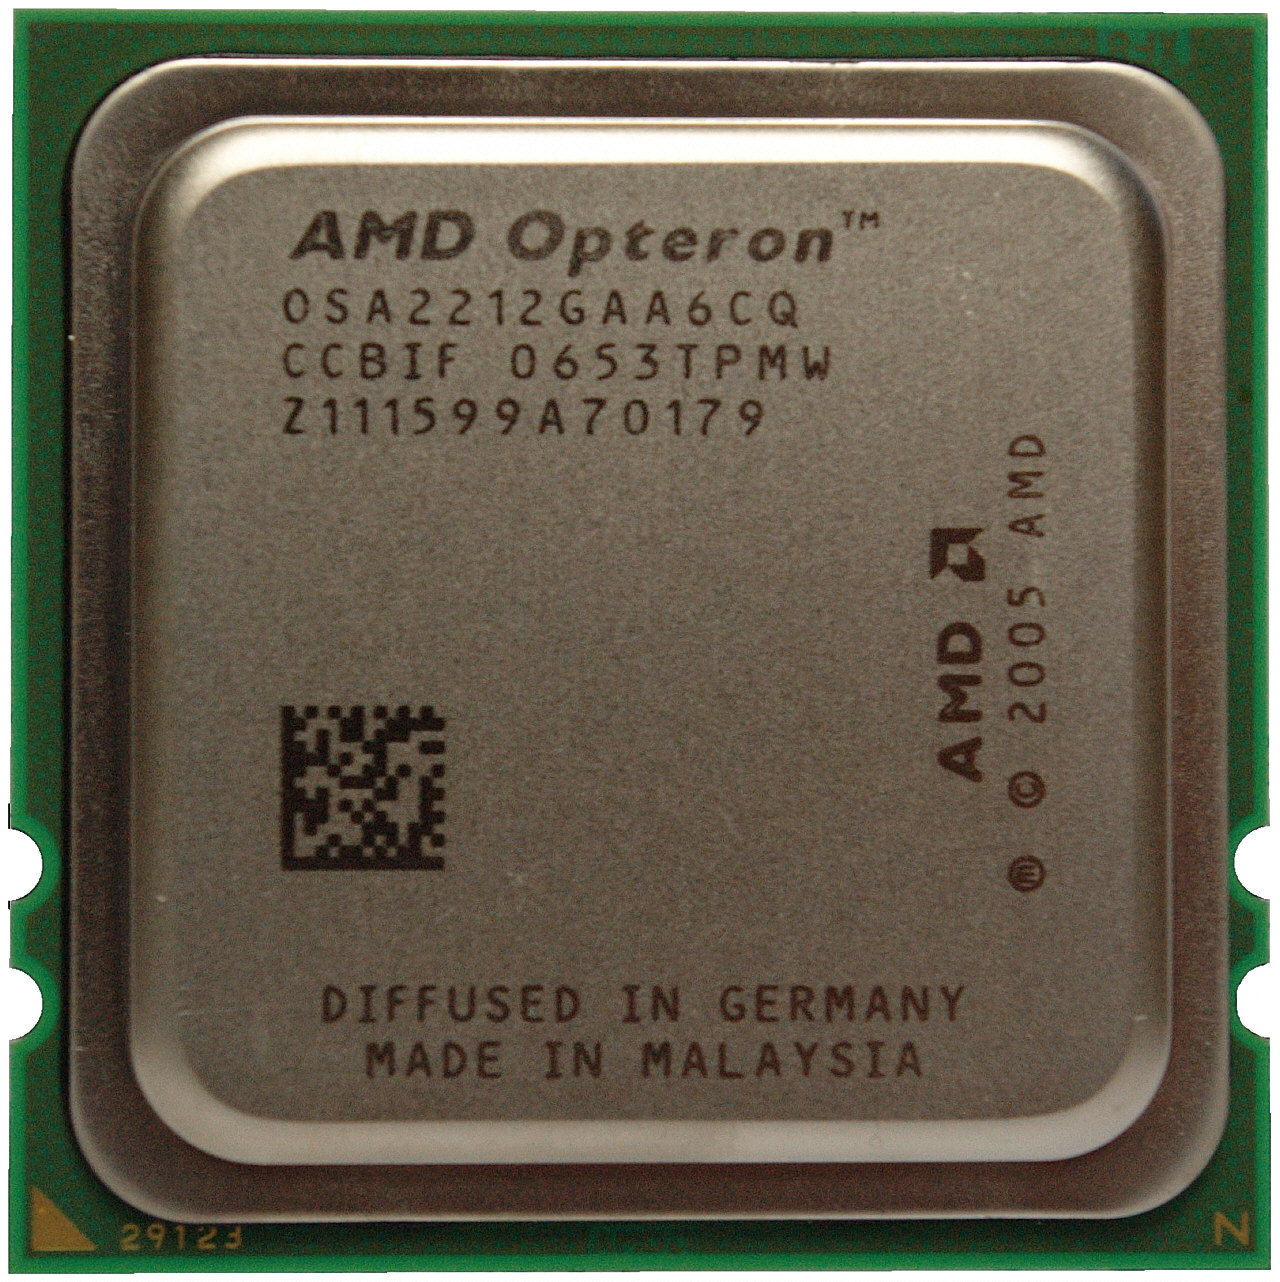
\includegraphics[height=0.1\textheight]{AMD_Opteron_2212_IMGP1795.jpg}
            \ent{center}
            \textcolor{gray}{\scriptsize{Rainer Knäpper, Free Art License (\url{artlibre.org/licence/lal/en/})}}
        \end{column}
    \begin{columns}
    \begin{itemize}{Aktueller (Juni 2016) Platz 3 Titan XK7 in der Top 500:}
        \item 18 688 AMD Opteron 6274 (16 Kerne) (140\,TDPFLOPS)
        \item 18 688 Nvidia Tesla K20X (1.3\,TDPFLOPS)  % (90% der Rechenlast)
    \end{itemize}
    % Ist eigtl. eher general knowledge, aber kann ja nicht schaden, als kleiner Einstieg, außer wenn ich dadurch ein Halbwissen zur Schau stelle.
    \begin{itemize}{General Purpose Graphical Processing Units(GPGPU) im Vergleich Prozessoren.}
        \item[+] Kosteneffektiv in Anschaffung
        \item[+] sehr gute Leistungsaufnahme pro GFlops
        \item[-] nur für bestimmte Anwendungen geeignet
            % sagen:
            %  - niedrig Latenz, streaming (in Bezug auf Speicehrzugriffe)
            %    (wenige random access)
            %  - eher für compute-bound (auf CPU) Probleme geeignet
        \item[+] hohe Speicherbandbreiten
        \item[-] niedrige Speicherlatenzen
        \item[+] Massiv parallel (3840 CUDA cores gegen 24 cores Xeon E7-8890-v4 (AVX2)
            % (Broadwell 14nm) http://ark.intel.com/products/91317/Intel-Xeon-Processor-E5-2699-v4-55M-Cache-2_20-GHz
            % http://ark.intel.com/de/products/93790/Intel-Xeon-Processor-E7-8890-v4-60M-Cache-2_20-GHz
            % http://www.cpu-world.com/info/id_model/Intel-server-conventions.html
            %   E7: Mission-critical
            %   v4: Broadwell
            % Broadwell AVX2 (256-Bits => 8 floats) (FMA*2) => entspricht also 24*8*2 CUDA-Cores = 384 -> Faktor 10 langsamer (meist nochmal Faktor 2 wegen kleiner Taktfrequenz von GPUs). Faktor 10,5 stimmt gut mit empirischen Messungen überein.
        \item[-] \textbf{zusätzliche Komplexität beim Programmieren}
    \end{itemize}
    % sagen:
    %  - Ziel dieser Belegarbeit ist es den letzten Punkt zu tilgen, indem man Berechnungen auf GPUs in das Spark-Framework einbringt (in nächsten Folien dann klar machen, dass die high-level Befehle in Spark sehr praktisch sind, um die GPU-Programmierung zu verstecken (map reduce abstraktion))
\end{frame}



%%%%%%%%%%%%%%%%%%%%%%%%%%%%%%%%%%%%%%%%%%%%%%%%%%%%%%%%%%%%%%%%%%%%%%%%%%%%%%%%
\section{Spark}
%%%%%%%%%%%%%%%%%%%%%%%%%%%%%%%%%%%%%%%%%%%%%%%%%%%%%%%%%%%%%%%%%%%%%%%%%%%%%%%%

% Following:
%  - https://www.toptal.com/spark/introduction-to-apache-spark
%  - "Learning Spark" book

\begin{frame}
    \frametitle{Spark Übersicht}
    % Sagen:
    %  - 2009 als Forschungsprojekt am UC Berkely Lab angefangen
    %  - 2013 Transfer zur Apache Software Foundation
    %  - GraySort Gewinner 5.11.2014: Apache Spark von Reynold Xin (Databricks Inc.)
    %     => 3x schneller bei 1/10 Knoten und 1/5 Datendurchsatz als alter Hadoop MapReduce-Gewinner
    %     => ab da wsl. richtig an Fahrt gewonnen
    Nachfolger zu Hadoop MapReduce. Geschrieben in Scala.
    % (Hadoop: Core MapReduce + verteiltes Dateisystem(HDFS,NFS,...))
    \begin{itemize}{Vorteile gegenüber von Hadoop MapReduce:}
        \item[+] Kann im Arbeitsspeicher arbeiten % , was Hadoop nicht anbot
        \item[+] Stellt viele Komplexbefehle zur Verfügung
        \item[+] iterative Algorithmen schneller als Hadoop wegen cache/persist-Funktionen
            % auch auf der Festplatte schneller als Hadoop MapReduce! % WARUM?!
            % http://stackoverflow.com/questions/26870537/spark-what-is-the-difference-between-cache-and-persist
            % cache only memory <-> persist can specify, e.g. disk
        \item[+] interaktive Konsole % zum schnellen Prototyping
        % vereinfachtere Programmierung gegenüber simplen MapReduce
        %   -> siehe nächste Folie
        \item[+] Unterstützung für: Scala, Java, Python, \ldots
        \item[+] Im Gegensatz zu zu Hadoop MapReduce auch lokales Dateisystem nutzbar % (Hadoop erzwingt HDFS), HDFS u.a. auch in Spark möglich
    \end{itemize}
\end{frame}


\begin{frame}
    \frametitle{Spark Anwendungen}
    % - datenanalyse, -visualisierung, prognosemodelle (z.B. "you also might like these products ...")
    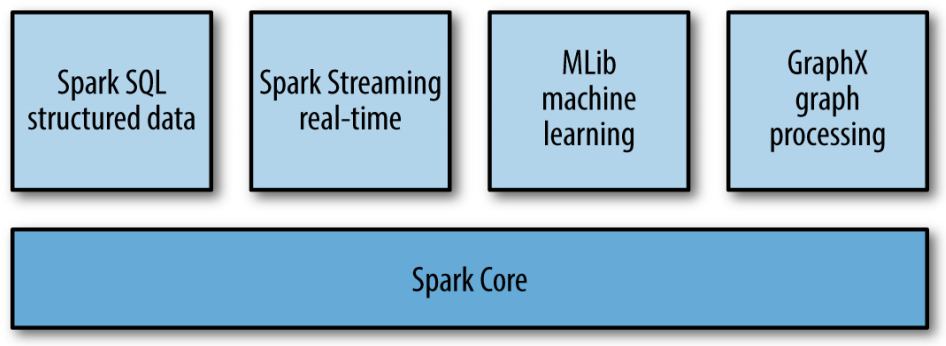
\includegraphics[width=0.8\linewidth]{spark-libraries.png}
    % sagen:
    %   - Spark SQL:
    %       - allow access to RDDs using SQL queries über einen SQL Kontext:
    %           val schemaString = "name age"
    %           ...
    %           val rowRDD = people.map(_.split(",")).map(p => Row(p(0), p(1).trim))
    %           val peopleDataFrame = sqlContext.createDataFrame(rowRDD, schema)
    %           val results = sqlContext.sql("SELECT name FROM people")
    %       http://spark.apache.org/docs/latest/sql-programming-guide.html#programmatically-specifying-the-schema
    %
    %   - Spark Streaming: Echtzeitdatenanalyse (z.B. Themen / häufigste Wörter in den letzten 10k Tweets). oder Kombination mit MLib möglich (Streaming Linear Regression)
    %     Data fitting während daten gestreamt werden (ich stelle mir z.B. least square fitting von einem physikalischen Experiment vor, z.B. v(t) fitting auf v(t)=v0+g*t fitting, um die Fallbeschleunigung g zu bestimmen, während gemessen wird. (Minimalbeispiel, denkbarer wäre wohl irgendetwas am LHC, mit ihren Terabyte an Daten pro Sekunde) -> Vorteil, dass die Daten nicht gespeichert werden müssen, was vlt. gar nicht möglich wäre:
    %           http://spark.apache.org/docs/latest/mllib-linear-methods.html#streaming-linear-regression
    %
    %   - MlLib: statistiken (mittelwert, standardabweichung, ...), korrelaton, (lineare) regression, k-means, stochastic(online) gradient descent ...
    %       http://spark.apache.org/mllib/
    %       http://spark.apache.org/docs/latest/ml-guide.html
    %       http://spark.apache.org/docs/latest/mllib-optimization.html
    %     Primitiven für Machinenlernen, aber keine highlevel abstraktion wie z.B. Keras, wo das Training in einer Zeile geht:
    %            model.fit( X_train, y_train,
    %                       nb_epoch=1000, batch_size=100,
    %                       verbose=1, validation_split=0.2,
    %                       callbacks=[EarlyStopping( monitor='val_loss',
    %                                                 patience=25, mode='min'),
    %                       WeightLogger()] )
    %               www.thoughtly.co/blog/deep-learning-lesson-3/
    %       (verstehe ich das so richtig ???)
    %       http://www.kdnuggets.com/2015/12/spark-deep-learning-training-with-sparknet.html
    %
    %   - GraphX
    %       Graphdatentyp + Algorithmen drauf wie
    %           PageRank: Berechnung der Relevanz / Popularität aller Knoten in einem Graphen aus den Wertungen ihrer jeweiligen Kanten
    %           subgraph ...
    %       http://spark.apache.org/docs/latest/graphx-programming-guide.html#graph_algorithms
\end{frame}


\begin{frame}
    \frametitle{Spark auf Github}
    \url{github.com/apache/spark.git master}\\
    % sagen:
    %   - anhaltende >aktive< Entwicklung (nicht wie Rootbeer ...)
    %   - 2012 nur 20k Code, nun 1 Millionen Zeilen -> betonen, um zu zeigen, dass es ein komplexes Projekt ist, für dass ein Mitwirken (GPU Plugin) möglicherweise den Rahmen einer Belegarbeit sprengt ... :)"
    %   - über tausend (1203 an 2016-07-06) Beitragende / Programmierer (210 in den letzten 30 Tagen)
    %   - 33 417 commits
    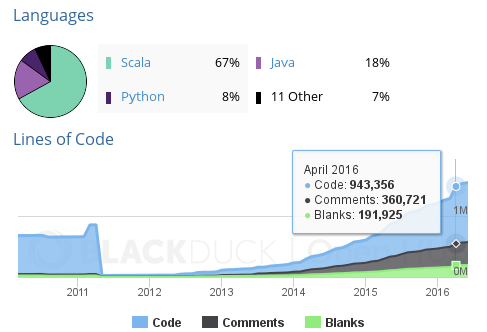
\includegraphics[width=\linewidth]{spark-openhub.png}\\
    \textcolor{gray}{\scriptsize{\url{
        https://www.openhub.net/p/apache-spark
    }}}
    % git://github.com/apache/spark.git master
\end{frame}


\begin{frame}
    \frametitle{MapReduce Programmiermodell}
    % nicht sicher in welchen Zitationsstil ich das hier machen soll, oder einfach nur freihand?
    - 2008: Paper ''MapReduce: Simplified Data Processing on Large Clusters'' von Jeffrey Dean und Sanjay Ghemawat (Google Inc.)
    %@article{
    %    author     = {Dean, Jeffrey and Ghemawat, Sanjay},
    %    title      = {MapReduce: Simplified Data Processing on Large Clusters},
    %    journal    = {Commun. ACM},
    %    issue_date = {January 2008},
    %    volume     = {51},
    %    number     = {1},
    %    month      = jan,
    %    year       = {2008},
    %    issn       = {0001-0782},
    %    pages      = {107--113},
    %    numpages   = {7},
    %    url        = {http://doi.acm.org/10.1145/1327452.1327492},
    %    doi        = {10.1145/1327452.1327492},
    %    acmid      = {1327492},
    %    publisher  = {ACM},
    %    address    = {New York, NY, USA},
    %}
\end{frame}


\begin{frame}
    \frametitle{Resilient Distributed Datasets (RDDs)}
    \begin{itemize}
        \item zu bearbeitende Daten liegen in RDD-Objekten
        % sagen:
        %  - sind eine Abstraktion
        \item Methoden zur Verarbeitung der Daten
              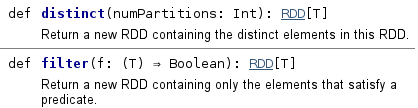
\includegraphics[scale=1.0]{rdd-disting-filter.png}
              \textcolor{gray}{\scriptsize{\url{
                 https://spark.apache.org/docs/0.8.1/api/core/org/apache/spark/rdd/RDD.html
              }}}
              % Bild soll für Programmierer zeigen, dass es wirklich nicht viel mehr als eine Klassenabstraktion ist, indem es Methoden dieser Klasse zeigt
        \item distributed
        \item resilient
    \end{itemize}
    % https://spark.apache.org/docs/1.5.2/api/scala/index.html#org.apache.spark.SparkContext
\end{frame}


%%%%NH: Nimm gleich das Monte Carlo Pi Beispiel statt wordcount
\begin{frame}
    Ermittlung der häufigsten Wörter in einem Text:

    \begin{lstlisting}[language=java]   % scala
        sc.
          textFile("./*").
          flatMap( line => line.split(" ") ).
          map( word => (word, 1) ).
          reduceByKey( (a, b) => a + b ).
          sortBy( _._2, false /*descending*/ ).
          take(500).
          foreach( println )
    \end{lstlisting}

    % Vergleich Hadoop MapReduce word count:
    %   https://hadoop.apache.org/docs/current/hadoop-mapreduce-client/hadoop-mapreduce-client-core/MapReduceTutorial.html#Example:_WordCount_v1.0
    % https://hadooptutorial.wikispaces.com/Sorting+feature+of+MapReduce
    % mit Spark version:
    %

    % Top 4:
    %  (ich,57766)
    %  (die,47869)
    %  (und,47663)
    %  (das,38866)
\end{frame}

\begin{frame}
    \frametitle{Spark Monte-Carlo Pi-Berechnung}
    \begin{lstlisting}{language=shell}
        $SPARK_ROOT/bin/spark-shell --master local[*]
    \end{lstlisting}
\end{frame}

% Was ist Spark, warum will ich es nehmen
% Wie funktioniert Spark ( RDD, Reduce, Slurm )
% Ein Beispiel mit Spark ( Monte Carlo und/oder word count -> chat log :) )

% \begin{frame}
% \begin{lstlisting}[language=bash]
% jobid=$(sbatch "$@" --output="$SPARK_LOGS/%j.out" --error="$SPARK_LOGS/%j.err" $HOME/scaromare/start_spark_slurm.sh)
% jobid=${jobid##Submitted batch job }
%
%
% function startSpark() {
%     export SPARK_LOGS=$HOME/spark/logs
%     mkdir -p "$SPARK_LOGS"
%     if [ ! -d "$SPARK_LOGS" ]; then return 1; fi
%     jobid=$(sbatch "$@" --output="$SPARK_LOGS/%j.out" --error="$SPARK_LOGS/%j.err" $HOME/scaromare/start_spark_slurm.sh)
%     jobid=${jobid##Submitted batch job }
%     echo "Job ID : $jobid"
%     # looks like: 16/05/13 20:44:59 INFO MasterWebUI: Started MasterWebUI at http://172.24.36.19:8080
%     echo -n "Waiting for Job to run and Spark to start.."
%     MASTER_WEBUI=''
%     while [ -z "$MASTER_WEBUI" ]; do
%         echo -n "."
%         sleep 1s
%         if [ -f $HOME/spark/logs/$jobid.err ]; then
%             MASTER_WEBUI=$(sed -nE 's|.*Started MasterWebUI at (http://[0-9.:]*)|\1|p' $HOME/spark/logs/$jobid.err)
%         fi
%     done
%     echo "OK"
%     export MASTER_WEBUI
%     export MASTER_ADDRESS=$(cat ~/spark/logs/${jobid}_spark_master)
%     function sparkSubmit() {
%         ~/spark-1.5.2-bin-hadoop2.6/bin/spark-submit --master $MASTER_ADDRESS $@
%     }
%     cat "$SPARK_LOGS"/$jobid.*
%     echo "MASTER_WEBUI   : $MASTER_WEBUI"
%     echo "MASTER_ADDRESS : $MASTER_ADDRESS"
% }
% export -f startSpark
%
% \end{frame}

%%%%NH: Was willst du mit dem folgenden sagen? Wie Spark auf einer GPU Partition gestartet wird? Lieber später diskutieren ...
startSpark --time=04:00:00 --nodes=$((nodes+1)) --partition=gpu2 --gres=gpu:$gpusPerNode --cpus-per-task=$coresPerNode
sparkSubmit ~/scaromare/MontePi/singleNode/singleGpu/multiGpuTestSpark/MontePi.jar \
                 $((nPerSlice*nSlices)) $nSlices $gpusPerNode 2>/dev/null |
                 tee tmp.log | tee -a "$fname-gpu.log"



%%%%%%%%%%%%%%%%%%%%%%%%%%%%%%%%%%%%%%%%%%%%%%%%%%%%%%%%%%%%%%%%%%%%%%%%%%%%%%%%
\section{Rootbeer}
%%%%%%%%%%%%%%%%%%%%%%%%%%%%%%%%%%%%%%%%%%%%%%%%%%%%%%%%%%%%%%%%%%%%%%%%%%%%%%%%
%%%%NH: hier eine Einführung Rootbeer (Paper referenzieren + kurz erklären -> insb. mit Übersetzung in 3 adress code etc. ..)

\begin{frame}
%%%%NH: die folgenden Punkte finde ich gut, aber lieber am Schluss des Results-Kapitel einfügen. Kannst ja auch deine contributions+deren Effekt rootbeer erwähnen.
%%%%NH: multi gpu fähigkeiten von rb erwähnen

% sagen:
%  - Leider wurde die meiste Bearbeitungszeit für diesen Beleg vom Lösen von Bugs beansprucht, sodass ich nicht darauf verzichten kann, zumindest einige davon zu erwähnen, auf dass sie jemanden helfen mögen, der einen ähnlichen Ansatz wie ich verfolgen möchte
Rootbeer zu beachten:
  - Bei dem Versuch Rootbeer mit Java 8 zu benutzen, kommt es zu
        java.lang.NullPointerException
            at soot.rbclassload.RootbeerClassLoader.loadHierarchySootClasses(RootbeerClassLoader.java:963)
    Nur Java 6 ist offiziell unterstützt, aber Java 7 scheint auch zu funktionieren
    % https://github.com/pcpratts/rootbeer1/issues/175 - Issues with jre1.8
  - GCC 4.9 nur unterstützt (wegen CUDA-Compiler)
  - Kaum neue Commits auf Github seit Juni 2015
    % https://github.com/pcpratts/rootbeer1/commits/master
  - Die option '-computecapability=sm_30' ist Pflicht, da seit CUDA 7.0 die Standardarchitektur "compute_12" nicht mehr unterstützt wird (korrekt nun "sm_12")
        nvcc fatal   : Unsupported gpu architecture 'compute_12'
    % https://github.com/pcpratts/rootbeer1/issues/180 - CUDA 7.0: nvcc fatal: Unsupported gpu architecture 'compute_12'
  - Automatische Kernel-Konfiguration hat einen Bug, der standardmäßig immer so viele Kernel startet wie gleichzeitig auf einem Shared Multiprozessor laufen können.
    % return new ThreadConfig( block_shaper.getMaxThreadsPerBlock(), 1, 1,
    %                          block_shaper.getMaxBlocksPerProc(), 1,
    % https://github.com/pcpratts/rootbeer1/issues/168
  - Bug wo Rootbeer hat standardmäßig versucht den gesamten freien Speicher minus den benötigten zu alloziieren versuchte
    % sagen:
    %  - verhinderte multi-GPU, weil ein Kontext schon so gut wie den gesamten Speicher für sich beanspruchen wollte.
    %  - nur ein Problem mit multiple Rootbeer.jar
    % https://github.com/mxmlnkn/rootbeer1/commit/0d9699a40b06a7e5efee7213ca7fb215d6ef1377
    % https://github.com/mxmlnkn/rootbeer1/commit/cc2318673077a52f13a8c4b4d294fbd39e639ca5
    % /media/d/Studium/9TH SEMESTER/scaromare/MontePi/multiNode/multiGpu/scala$ /opt/spark-1.5.2/bin/spark-submit --master local[4] --class TestMonteCarloPi MontePi.jar 268435456 2
    %   16/01/22 03:27:59 ERROR Executor: Exception in task 1.0 in stage 0.0 (TID 1)
    %rg.trifort.rootbeer.runtime.CudaErrorException: CUDA_ERROR_OUT_OF_MEMORY: Error in cuMemAlloc: gpu_object_mem
    %   at org.trifort.rootbeer.runtime.CUDAContext.nativeBuildState(Native Method)
    %   at org.trifort.rootbeer.runtime.CUDAContext.access$1100(CUDAContext.java:17)
    %   at org.trifort.rootbeer.runtime.CUDAContext$GpuEventHandler.onEvent(CUDAContext.java:315)
    %   at org.trifort.rootbeer.runtime.CUDAContext$GpuEventHandler.onEvent(CUDAContext.java:308)
    %   at com.lmax.disruptor.BatchEventProcessor.run(BatchEventProcessor.java:128)
    %   at java.util.concurrent.ThreadPoolExecutor.runWorker(ThreadPoolExecutor.java:1145)
    %   at java.util.concurrent.ThreadPoolExecutor$Worker.run(ThreadPoolExecutor.java:615)
    %   at java.lang.Thread.run(Thread.java:745)
  - die ausführbare jar für Spark darf kein Leerzeichen im Pfad enthalten:
    % $SPARK_ROOT/bin/spark-submit --master $MASTER_ADDRESS ./src/sort.py "$(pwd)"/data/The_Complete_Works_of_Willia.txt
    %   java.io.FileNotFoundException: Added file file:/media/f/Studium/9TH%20SEMESTER/scaromare/spark-gpu/src/sort.py does not exist.
    %      at org.apache.spark.SparkContext.addFile(SparkContext.scala:1365)
%  - Alignement Bug in Speicherserialisierung
%       https://github.com/mxmlnkn/rootbeer1/commit/cc2318673077a52f13a8c4b4d294fbd39e639ca5
  - Zu kompilierende jar an Rootbeer >muss< auf .jar enden
    % normalerweise sollte die Dateiendung unter Linux egal sein, gibt Magic Bytes und Co
    % #Warning: the following soot-classpath entry is not a supported archive file (must be .zip, .jar or .apk): MontePiGPU.jar.tmp
\end{frame}

\begin{frame}
Scala GPU:
  - ScalaCL ( "ScalaCL is not production-ready!" )
  - BIDMach
  - Firepile
  - Rootbeer (
\end{frame}

\begin{frame}
Run on Taurus:
    module load java/jdk1.7.0_25 scala/2.10.4 cuda/7.0.28
    # manuelle Installation von maven, ant, spark, zipmerge
    % für spark wurden precompiled binaries genommen, weil es bei der Kompilation auch Probleme gab, die nicht behoben werden konnten
    export PATH="$PATH:$HOME/spark-1.5.2-bin-hadoop2.6/bin/:$HOME/spark-1.5.2-bin-hadoop2.6/sbin/:$HOME/programs/bin"
\end{frame}

\begin{frame}
    \frametitle{Rootbeer Funktionsweise}
    3.) Rootbeer constructor
    3.1.) CUDALoader constructor
    3.2.) CUDALoader.load
          Load shared libraries with fixed absolute paths mostly ...
              m_libCudas.add("/usr/lib64/libcuda.so");
              m_libCudas.add("/usr/lib/x86_64-linux-gnu/libcudart.so.5.0");
              m_rootbeerRuntimes.add(RootbeerPaths.v().getRootbeerHome()+"rootbeer_x64.so.1");
              m_rootbeerCudas.add(RootbeerPaths.v().getRootbeerHome()+"rootbeer_cuda_x64.so.1");
    4.) Rootbeer.getDevices
          Class c = Class.forName("org.trifort.rootbeer.runtime.CUDARuntime");
          Constructor<IRuntime> ctor = c.getConstructor();
          m_cudaRuntime = ctor.newInstance();
          m_cards.addAll( m_cudaRuntime.getGpuDevices() );
    4.1.) CUDA_Runtime.c
            status = cuDeviceGet(&device, i);
            cuDeviceGetAttribute(...)
            [...]
    5.) GPUDevice.createContext -> CUDAContext -> native initializeDriver
            https://de.wikipedia.org/wiki/Java_Native_Interface
        ./csrc/org/trifort/rootbeer/runtime/CUDAContext.c:JNIEXPORT void JNICALL Java_org_trifort_rootbeer_runtime_CUDAContext_initializeDriver
            only saves function pointers to context.java
    6.) Rootber.run
    6.1.) Context context = createDefaultContext(); // skipped for multi-GPU
    6.2.) context.setThreadConfig(thread_config);
    6.3.) context.setKernel(work.get(0));
    6.4.) context.setUsingHandles(true);
    6.5.) context.buildState();
            gpuEvent.setValue(GpuEventCommand.NATIVE_BUILD_STATE);
                GpuEventHandler.onEvent
                    nativeBuildState( ..., gpuDevice.getDeviceId(), ... )
                        Java_org_trifort_rootbeer_runtime_CUDAContext_nativeBuildState in CUDAContext.c
    6.6.) context.run(work)
            context.runAsync(work)
                gpuEvent.setValue(GpuEventCommand.NATIVE_RUN_LIST);
                    GpuEventHandler.onEvent
                        writeBlocksTemplate();
                        runGpu();
                            cudaRun(nativeContext, objectMemory, b2i(!usingHandles), stats);
                        readBlocksTemplate();
          private native void cudaRun(long nativeContext, Memory objectMem, int usingKernelTemplates, StatsRow stats);

Rootbeer-Paper:
        1) serialize state to GPU memory
        2) define the kernel code that the GPU will execute
        3) control the kernel
        4) deserialize state back to CPU memory
      -> "serialize"?
      => Rootbeer does these things automatically in contrast to CUDA- and OpenCL- Java language bindings
      supports:
        1) single and multi-dimensional arrays of primitive and reference types
        2) composite objects
        3) instance and static fields
        4) dynamic memory allocation
        5) inner classes
        6) synchronized methods and monitors
        7) strings
        8) exceptions that are thrown or caught on the GPU
    Introduction
      - focus on NVidia because of recursion
      - Without Rootbeer, using Java language bindings, a developer must carefully convert complex graphs of Java objects into arrays of basic types.
      - Without Rootbeer, a developer must write separate code in another language to specify what the GPU execution will do
      - Rootbeer also has a native debugging mode where the GPU code is executed on a multi-core CPU inside a C++ debugger.
    Programming Interface:
        public interface Kernel {
            void gpuMethod();
        }
      - get data onto GPU by settings private members
      - byte code from gpuMethod is cross-compiled with CUDA
        List<Kernel> jobs = new ArrayList<Kernel>();
        int[] ret = new int[ arrays.size() ];
        for( int i = 0; i < arrays.size(); ++i )
        {
            jobs.add( new ArraySum( arrays.get(i), ret, i ) );
        }
        Rootbeer rootbeer = new Rootbeer();
        rootbeer.runAll(jobs);
      - compile to jar
      - run Rootbeer on jar
        java -jar Rootbeer.jar InputJar.jar OutputJar.jar
    High Level Processing Overview:
      - jar -[extract]-> .class
            -[read with Soot]-> Jimple:
         . search for Kernel implementations
         . find all types, methods, fields meant for GPU
            -[generated CUDA code]-> .cu
            -[call nvcc]-> .cubin
         . Generate byte code for serialization
         . insert compiled interface which serialzes and calls cubin
           -> convert back to bytecode
        -[pack into jar]-> jar
    High Performance (De)Serialization in Java
        1) Java Native interface (JNI)  247 ms
        2) Reflection                   173 ms
        3) Purve Java                     5 ms
      - "custom Java Bytecode that reads fields and places the results into a Java byte array"
          -> scheint komplett zerstreut im Speicher zu liegen ...
       -> JNI call cudaMemcpy
    Representing Java Objects on the GPU
      - static + instance memory
         |              |
         + simple C-Array with differing offsets (must be primitive type)
                        +
            set of object with 16B header:
                Reserved for Garbage Collector 10 bytes (future work)
                Derived Type                    1 byte
                Created on GPU flag             1 byte  (malloc from kernel)
                Object Monitor State            4 bytes
    CUDA Code Generation:
      - Future: better serialization + shared memory
    Related Work:
      - jCUDA, jocl, JavaCL -> require serialization of object graphs to primitive arrays
      - JikesRVM to auto-detect parallelism runtime
      - Peter Calvert’s annotations like OpenMP -> not well-working for all cases ...
      Aparapi very similar, but less full-featured
\end{frame}

%%%%NH: gibt es beschränkungen, welche funktionen implementiert werden können oder ist die geschichte turing-vollständig?


%%%%%%%%%%%%%%%%%%%%%%%%%%%%%%%%%%%%%%%%%%%%%%%%%%%%%%%%%%%%%%%%%%%%%%%%%%%%%%%%
\section{Implementation}
%%%%%%%%%%%%%%%%%%%%%%%%%%%%%%%%%%%%%%%%%%%%%%%%%%%%%%%%%%%%%%%%%%%%%%%%%%%%%%%%


\begin{frame}
    \frametitle{Zuordnung der Grafikkarten zu Partitionen}
    - momentan eher gehackter Ansatz, mit manuell geschriebenen Distributor und der Beobachtung, dass Partition in einer bestimmten Weise auf Knoten gemappt werden:
    % startSpark --time=04:00:00 --nodes=5 --partition=west --gres= --cpus-per-task=12
    % spark-shell --master=$MASTER_ADDRESS
    % scala> import java.net.InetAddress
    % scala> sc.parallelize( 1 to 5*12, 5*12 ).map( (x) => { Thread.sleep(10); x+" : "+InetAddress.getLocalHost().getHostName() } ).collect().foreach( println )
    Partition Hostname
         1 : taurusi3164
         2 : taurusi3165
         3 : taurusi3167
         4 : taurusi3166
         5 : taurusi3164
         6 : taurusi3165
         7 : taurusi3167
         8 : taurusi3166
         9 : taurusi3164
        10 : taurusi3165
        11 : taurusi3167
        12 : taurusi3166
        13 : taurusi3164
        14 : taurusi3165
        15 : taurusi3167
        16 : taurusi3166
     also interleaved:
        Partion mod (nKnoten=4) = 1 -> taurusi3164
        Partion mod (nKnoten=4) = 2 -> taurusi3165
\end{frame}



%%%%%%%%%%%%%%%%%%%%%%%%%%%%%%%%%%%%%%%%%%%%%%%%%%%%%%%%%%%%%%%%%%%%%%%%%%%%%%%%
\section{Performanceanalyse}
%%%%%%%%%%%%%%%%%%%%%%%%%%%%%%%%%%%%%%%%%%%%%%%%%%%%%%%%%%%%%%%%%%%%%%%%%%%%%%%%

%%%%NH: hardware auf der du deine tests durchgeführt hast beschreiben
%%%%NH: nochmal kurz den benchmark + motivation beschreiben  (use case => machine learning in labs). auch erwähnen, dass du eine cuda implementation erstellt hast ..
%%%%NH: spannend wäre, ob bottlenecks in der implementierung => allg. profiling von spark/rootbeer code // hast du bottlenecks entdeckt?

\begin{frame}
    Einkernleistungsanalysen: %%%%NH: was bedeutet 1 Kern: 1 Core? 1 Node? 1 GPU?
    % Erstellt  mit:
    %   ssh taurus
    %   # Rootbeer commit ef79eaddc7956bf9bb3b9bd4d287e377e3949075
    %   ( git checkout a2302ec67b3f96df &&
    %     cd ~/scaromare/rootbeer1/csrc &&
    %     ./compile_linux_x64           &&
    %     cd ..                         &&
    %     ant jar                       &&
    %     ./pack-rootbeer )
    %   makeOpts=( \
    %       "SPARK_ROOT=$HOME/spark-1.5.2-bin-hadoop2.6" \
    %       "SPARKCORE_JAR=~/spark-1.5.2-bin-hadoop2.6/lib/spark-assembly-1.5.2-hadoop2.6.0.jar" \
    %       "SCALA_ROOT=$(dirname $(which scala))/../lib" \
    %   )
    %   cd ~/scaromare/MontePi
    %   git checkout
    %   make -B -C singleNode/singleCore/java/  "${makeOpts[@]}"  MontePi.jar
    %   make -B -C singleNode/singleCore/scala/ "${makeOpts[@]}"  MontePi.jar
    %   make -B -C singleNode/singleGpu/cpp/    "${makeOpts[@]}"  MontePi.jar
    %   make -B -C singleNode/multiGpu/java/    "${makeOpts[@]}"  MontePi.jar
    %   make -B -C singleNode/multiGpu/scala/   "${makeOpts[@]}"  MontePi.jar
    %   salloc -p gpu2-interactive --nodes=1 --ntasks-per-node=1 --cpus-per-task=1 --gres=gpu:1 --time=02:00:00
    %   ~/scaromare/MontePi/benchmarkImpl.sh
    %   cd scaromare/MontePi/
    %   python plot.py --workload-log 2016-07-02_01-18-12/results.log
    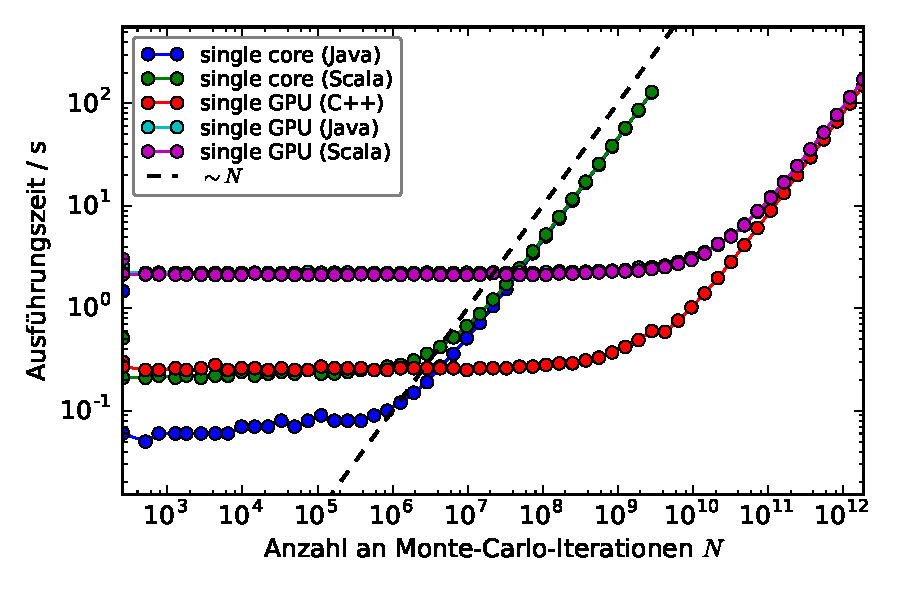
\includegraphics[width=0.8\linewidth]{benchmarks-workload-scaling.pdf}
    % sagen:
    %   - benchmarkImpl.sh misst mittels 'time' Linuxshellbefehls
    %   - overhead ist riesig, für GPU vs CPU und für Java vs. C++ -> relativ große Probleme rentieren sich nur
    %   - Java wird für sehr große Probleme schneller als C++ -> Vorteil der automatischen Optimierungen durch die JVM durch Rootbeer! -> nächste Seite Profiler nur kurz erwähnen
\end{frame}

%%%%NH: multi gpu, multi node single gpu, multi node multi gpu, ...

\begin{frame}
Profiling von Rootbeer ohne Spark mit dem NVIDIA Visual Profiler:
    srun -p gpu-interactive --nodes=1 --ntasks-per-node=1 --cpus-per-task=1 --gres=gpu:2 --time=1:30:00 --mem-per-cpu=6000 --x11=first nvvp
    Executable: /sw/global/tools/java/jdk1.7.0_25/bin/java
    Working Directory: ... ???
    Arguments: -jar ./MontePi.jar 2684354560
       -> works :3
 -> BILDER!
\end{frame}



%%%%%%%%%%%%%%%%%%%%%%%%%%%%%%%%%%%%%%%%%%%%%%%%%%%%%%%%%%%%%%%%%%%%%%%%%%%%%%%%
\section{Zusammenfassung}
%%%%%%%%%%%%%%%%%%%%%%%%%%%%%%%%%%%%%%%%%%%%%%%%%%%%%%%%%%%%%%%%%%%%%%%%%%%%%%%%
%%%%NH: Herr Nagel fragt gern: ``Was haben wir gelernt''
%%%%NH: => generell im Ausblick vielleicht noch erwähnen, was zukünftig (an deinem Framework, Rootbeer) verbessert werden sollte
%%%%NH: => z.B. gibt es möglichkeiten, um host-gpu transfers zu vermeiden/verringern
%%%%NH: verringerung der latenz durch einsatz neuer bustechnologien (nvlink)?
\begin{frame}
	\frametitle{Zusammenfassung}
	\begin{itemize}
		\item ...
	\end{itemize}
\end{frame}

%\appendix

\end{document}
